%%%%%%%%%%%%%%%%%%%%%%%%%%%%%%%%%%%%%%%%%%%%%%%%%%%%%%%%%%%%%%%%%%%%%%%%%%%%%%%%
%2345678901234567890123456789012345678901234567890123456789012345678901234567890
%        1         2         3         4         5         6         7         8
% THESIS Chapter

\chapter{Background}

\section{State of the Art}
\subsection{Dynamic visualisation}
\label{sec:sec21}
\subsubsection{Visualising the temporal element}
\label{sec:subsec21}
In 2014 an investigation was done into the state of the art of visualising the dynamic element or third dimension \cite{tsotaivg}. Whilst this report will focus on measure visualisations it can be useful to see how the temporal element was visualised at a network level and how this could be applied to measures. 

\subsubsection{The mental map}
\label{sec:subsec21}
Another key aspect to bear in mind is that the measure visualisations should build on, or at the very least not damage, the user's mental map of the dynamic graph. Preservation of the mental map feature is often cited as a desired criterion for a successful dynamic graph drawing algorithm \cite{tmitmmeridgd}. 

\subsection{Dynamic Measures}
\label{sec:sec22}
Dynamic measures fall into two categories. The first category is measures which only make sense in a dynamic context. The second is when static measures are applied and calculated at each time frame.

\subsubsection{Local Measures}
Local measures change depending on the time period specified and are localised to a node. 

\subsubsection{Global Measures}
Global measures are calculated on the graph as a whole.


\section{The Vistorian}
The Vistorian \cite{bach:hal-01205822} is an ongoing open source project by Benjamin Bach, Nathalie Henry Riche, Roland Fernandez, Emmanoulis Giannisakis, Bongshin Lee, et al to create an online platform which provides interactive visualization for various kinds of networks, designed for social scientists and historians. 

\section{Technologies}
\subsection{JavaScript and D3}
\label{sec:sec24}
The Vistorian was primarily written in TypeScript and D3 \cite{d3site}. Since I'm more comfortable working directly with Javascript all code was implemented using Javascript. D3 was used for the visualisations.

\section{Node-Link Diagrams}
\subsection{Background}
-Positions of nodes kept same for all diagrams, easier to visualise \cite{tsotaivg}.\newline
-Node-link is worse than matrix representation when over 20 nodes \cite{acotrogunlambr}.\newline
-Node-link history and development, why I'm using this one.\newline
-Basic and intuitive.\newline

\subsection{Vistorian Implementation}

\begin{center}
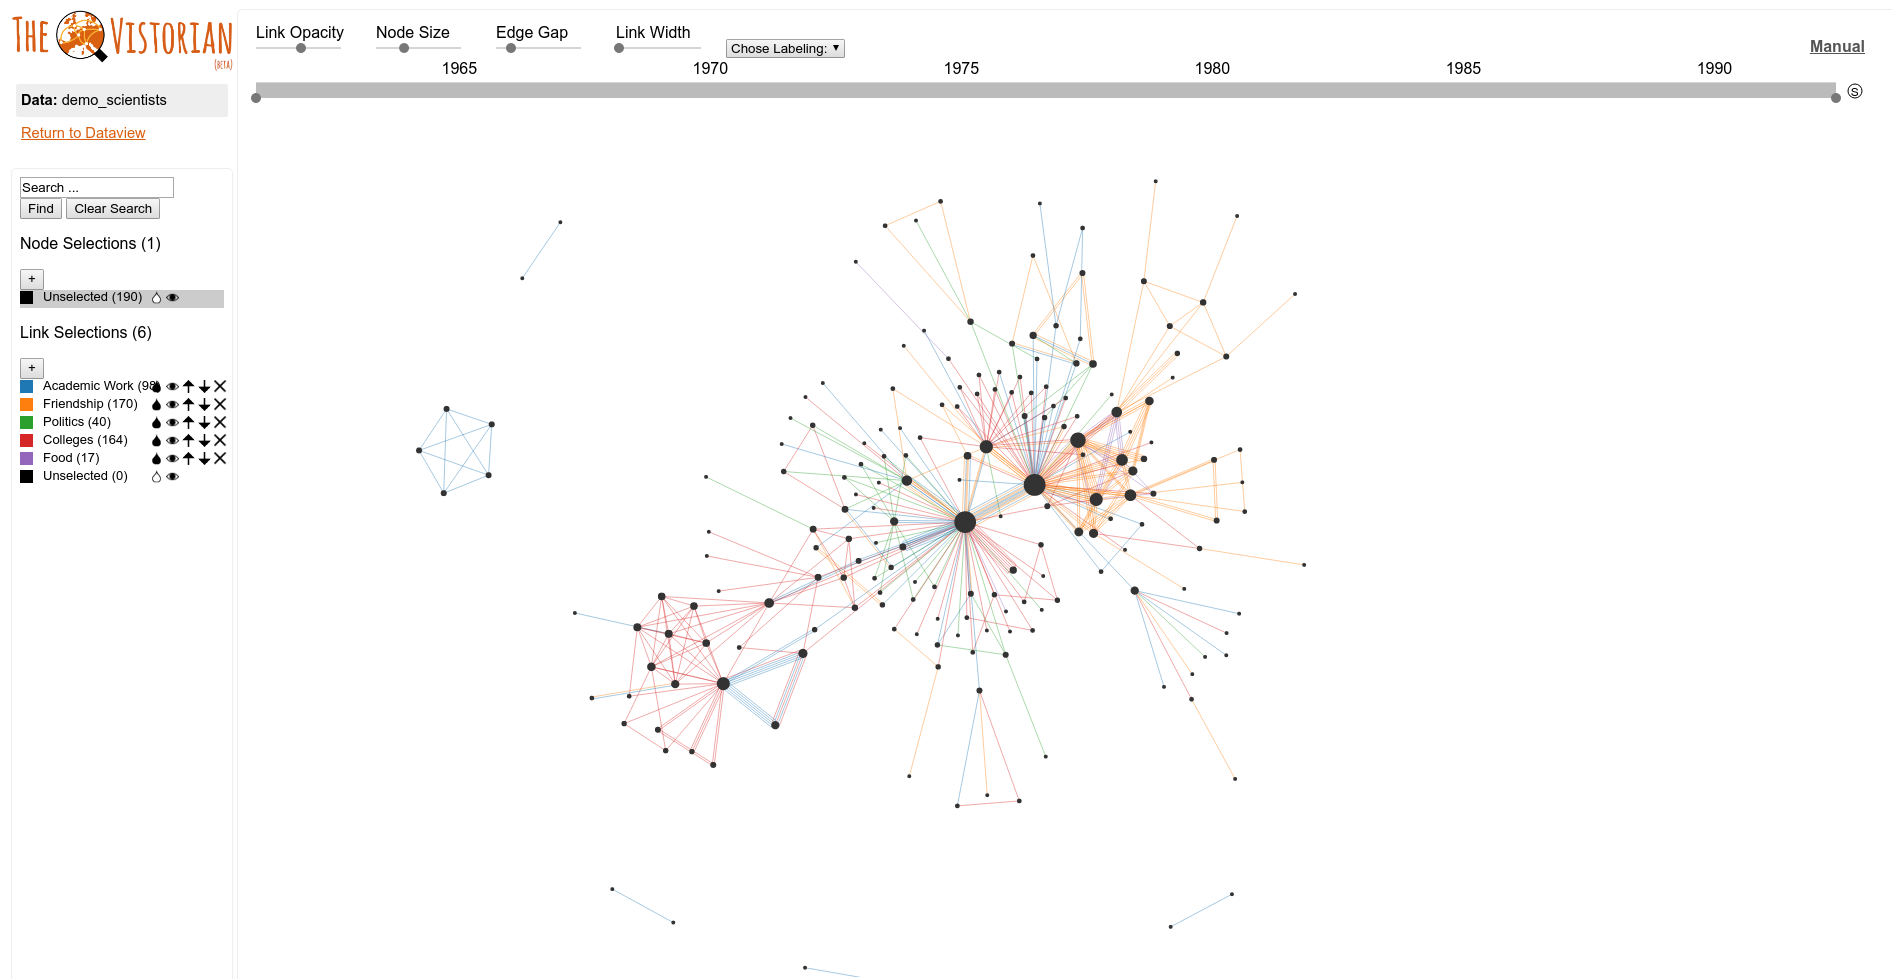
\includegraphics[trim={0 0 0 0}, width=140mm]{./Figures/vistorianOriginal.png}
\end{center}

More details are given in the visualization manual \cite{vismanual} but a summary of the key aspects is provided below.
This project will focus on the ‘Node-link’ visualisation specifically. The node-link diagram is composed of nodes as points and edges as straight lines. At the top of the network page is a time-slider. Adjusting this time slider filters the links shown if they are not present in that window. A force-directed layout is used, meaning that nodes with many common neighbours are drawn close to each other and nodes with fewer connections are moved to the edges. Node size is used to indicate the node degree and line colour indicates a specific type of relation.\newline
-mention edges vs nodepairs.\newline
-mention that edges in this case are messages being sent.


\section{Dynamic Nature}
The network has been split into 60 discrete steps/frames, which are the unit of change. Since the data is of letters being sent, having each time this happened be a step wouldn’t work well in terms of analysis (???). By having discrete steps we can ‘chunk’ the data and give more meaningful analysis over the longer term. (This is probably something to discuss with BB, I feel that this is maybe the right direction and something worth mentioning but it’s hard to correctly justify why.)








